\section{Workflow} % (fold)
\label{sec:workflow}
	Im folgenden Abschnitt soll erläutert werden wie ein moderner Workflow aussehen kann. Dabei sollen viele Aufgaben, die von vielen noch per Hand erfolgen, automatisiert werden.\\

	\subsection{Nodejs} % (fold)
	\label{sub:nodejs}
		Nodejs - ist eine auf Chromes Javascript runtime aufbauende Plattform. Wärend Server vor allem in PHP oder anderen Sprachen programmiert werden ist dies durch Nodejs auch mit Javascript möglich. Nodejs liefert einen eigenen Paket Manager namens "`npm"'.
	% subsection nodejs (end)

	\subsection{Node Package Manager} % (fold)
	\label{sub:node_package_manager}
		Auch als "`npm"' abgekürzt, erlaubt das installieren von Paketen mittels der Kommandozeile. Ein Beispiel:\\
		Das Paket "`tmi - too many images"' analysiert eine gegebene URL nach ihrer totalen Bildgröße und vergleicht es mit der durchschnittlichen größe des Webs. Es lässt sich mittels \texttt{npm}-Befehl über die Kommandozeile installieren:
		\begin{figure}[htbp]
			\begin{center}
				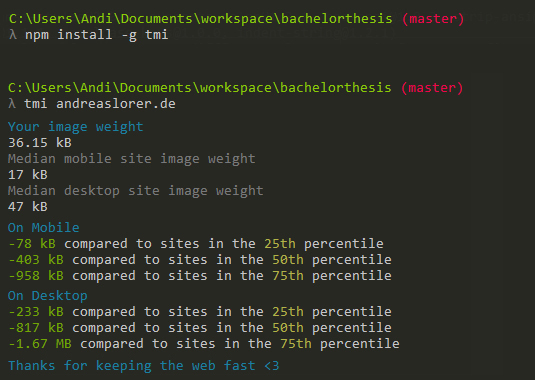
\includegraphics[width=0.7\textwidth]{npm_install_tmi.jpg}
				\label{fig:npm_install_tmi}
			\end{center}
		\end{figure}
		Danach lässt es sich ganz einfach per Befehl aufrufen:

		Es wäre aber auch möglich das unter Punkt \ref{ssub:google_pagespeed_insight} vorgestellte \texttt{Google Pagespeed Insight} mittels "`npm install -g psi"' zu installieren und per "`psi someURL.de"' aufzurufen. Es gibt bereits mehr als 134,082 Pakete (Stand 21.03.2015) die verschiedenste Aufgaben erledigen können. Das Spektrum an Paketen ist sehr groß und reicht von sinnlosen Aufgaben (wie dem zufälligen generieren von Katzennamen\footnote{Cat-names: \url{https://www.npmjs.com/package/cat-names}}) bis hin zu hoch komplexen Programmen wie "`sitespeed.io"'\footnote{Sitespeed.io: \url{http://www.sitespeed.io/}}, dass eine rekursive Performance-Analyse einer ganzen Webanwendung ermöglicht.\\

		\subsubsection{Dependency Management} % (fold)
		\label{ssub:dependency_management}
			Der klassische Weg wie externe Abhängigkeiten des Projekts geregelt werden sieht wie folgt aus:
			\begin{itemize}
				\item Zu Beginn des Projekts werden Bibliotheken und Frameworks heruntergeladen.
				\item Es folgt das Entpacken und das Verschieben in das richtige Projektverzeichnis.
				\item Erscheint beispielsweise eine neue Version des Frameworks beginnt dieser Prozess von neuem.
			\end{itemize}

			Dependency Manager (wie z.B. npm oder Bower\ref{ssub:bower}) schaffen hier Abhilfe. Durch Ausführen des Befehls: "`npm init"' lässt sich eine neue Abhängigkeitsstruktur für ein Projekt anlegen. Dabei wird eine Datei mit dem Namen: "`package.json"' erzeugt. In dieser Datei werden nun sowohl die Beschreibung, die Version als auch alle Abhängigkeiten gespeichert. Will man nun beispielsweise das Programm "`Gulp"' \ref{sub:task_manager_gulp} installieren, erfolgt dies ganz einfach über das Kommando:\\
			"`npm install -save gulp"'. Die \texttt{-save} Option bedeutet dabei, dass folgender Eintrag in die package.json Datei erfolgen soll:

			\begin{lstlisting}[captionpos=b, caption=, label=lst:]
{
  "dependencies": {
    "gulp": "^3.8.11"
  }
}
			\end{lstlisting}

			\texttt{\textasciicircum 3.8.11} bedeutet dabei, dass für dieses Projekt mindestens eine Gulp Version größer als 3.8.11 vorliegen muss. Der große Vorteil besteht nicht nur darin, dass weder ein Seitenaufruf erfolgt, noch die Dateien entpackt und verschoben werden müssen. Zudem lässt sich über den Befehl "`npm update"' alle Pakete auf die neuste Version bringen. Die package.json Datei lässt sich zudem in die Versionskontrolle einfügen. Der von npm angelegte Ordner: "`node\_modules"' sollte unbedingt per \texttt{.gitignore} von der Versionierung ausgeschlossen werden! Läd ein Teammitglied das Repository herunter, so muss nur noch "`npm install"' aufgerufen werden und alle Abhängigkeiten, mit den für dieses Projekt verwendeten Versionsnummern werden heruntergeladen und installiert. Damit ist jedes Teammitglied auf dem selben Stand und verwenden die selbe Version. Neue Abhängigkeiten lassen sich so auch ganz einfach an alle Mitglieder verteilen.			
			
		% subsubsection dependency_management (end)

		\subsubsection{Bower} % (fold)
		\label{ssub:bower}
			Wie \texttt{npm} so ist auch \texttt{Bower} ein Paket Manager. Um genau zu sein basiert Bower auf npm und lässt sich mittels "`npm install -save bower"' für das Projekt installieren. Der Vorteil von Bower besteht darin, dass über eine \texttt{.bowerrc} Datei angeben werden kann, in welchem Ordner die Pakete installiert werden sollen. Dies ist bei npm nicht möglich.\\
			Es lohnt sich Frameworks und Libraries wie z.B. \texttt{Bootstrap} oder \texttt{Underscore} mittels Bower zu installieren und andere Programme wie zum Beispiel Gulp oder Nodejs Module per npm.\\
			Bower lässt sich, ähnlich wie npm, über das Kommando: "`bower init"' Initialisieren. Danach lassen sich per Befehl "`bower install -save bootstrap"' das Bootstrap Framework installieren. 

			\begin{figure}[htbp]
				\begin{center}
					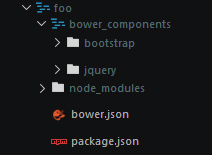
\includegraphics[width=0.3\textwidth]{bower_structure.jpg}
					\label{fig:bower_structure}
				\end{center}
			\end{figure}
			
			Wie zu sehen ist, wurde nicht nur Bootstrap von Bower installiert, sondern auch JQuery. Das liegt daran, dass Bootstrap als interne Abhängigkeit wiederrum auch Abhängigkeiten besitzt, die bei der Installation von Bootstrap gleich mit installiert werden. Entfernt man Bootstrap nun wieder, so würde auch JQuery entfernt werden. Würde Bootstrap in einer neuen Version erscheinen, die von einer höheren JQuery Version abhängt, so würde Bower automatisch auch JQuery auf die nötige Version aktualisieren.
		
		% subsubsection bower (end)

	% subsection node_package_manager (end)

	\subsection{Task Manager - Gulp} % (fold)
	\label{sub:task_manager_gulp}
		Warum und für was braucht es überhaupt einen Task Manager?
		\begin{quote}
			\textit{If you aren't using productivity tools or task automation, you are working \textbf{too hard.} [...] Automation isn't about being lazy. It's about being \textbf{efficient}.}\autocite[p. 18,78]{addyOsmani14}
		\end{quote}
		Ein Task Manager übernimmt immer wiederkehrende Arbeiten. Dazu zählt zum Beispiel die Aufgabe "`minify, uglify und concatenating"' wie in Punkte: \ref{ssub:ressourcen_reduzieren} bereits beschrieben. Aber auch das Übersetzen von "`Sass"'\footnote{Sass is the most mature, stable, and powerful professional grade CSS extension language in the world. \url{http://sass-lang.com}}, oder das optimieren und verkleinern von Bildern lassen sich als Task beschreiben und automatisieren.
		Die zwei bekanntesten Task Manager heißen \texttt{Gulp} und \texttt{Grunt}. Hier soll das Arbeiten mittels Gulp beschrieben werden, denn er ist sehr viel einfacher zu benutzen als Grunt.

		\begin{figure}[htbp]
			\begin{center}
				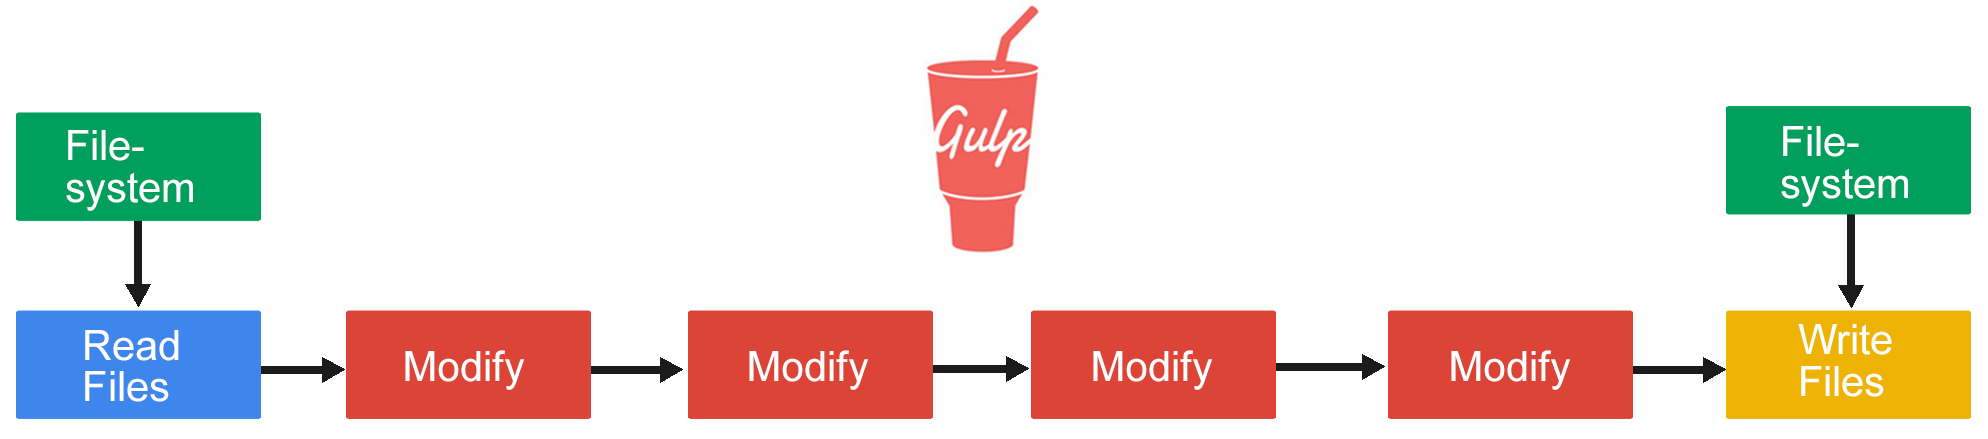
\includegraphics[width=\textwidth]{gulp.jpg}
				\caption{Gulp arbeitet nach dem "`file stream"' Prinzip (Eigene Abbildung nach \autocite[p. 85]{addyOsmani14})}
				\label{fig:gulp}
			\end{center}
		\end{figure}

		Gulp besteht nur aus 4 Kommandos:
		\begin{enumerate}
			\item gulp.task: Definiert einen Namen für einen Gulp Task. Dadurch wird dieser Task über die Kommandozeile benutzbar. Für Anwender die wenig mit der Kommandozeile arbeiten wollen gibt es auch eine Google Chrome Browsererweiterung namens Gulp-devtools. Damit lassen sich die verschiedenen Tasks ganz einfach über eine Benutzeroberfläche verwenden.
			\item gulp.src: Greift auf eine oder mehrere Dateien zu. Auch Ordner können angegeben werden.
			\item gulp.dest: Schreibt die Datei in den angegebenen Ort.
			\item pipe: Mittels "`pipe"' lassen sich die Dateien (auch file streams genannt) modifizieren. Dabei lässt sich pipe beliebig oft aufrufen. Die Aufgabe: "`minify, uglify und concatenating"' könnte dabei so erfolgen:
			\begin{lstlisting}[captionpos=b, caption=, label=lst:]
// require the gulp modules needed:
var gulp = require('gulp');
var uglify = require('gulp-uglify');
var concat = require('gulp-concat');

// javascript task: concat, minify, uglify all javascript files in folder:
gulp.task('javascript', function () {
    gulp.src(['site/assets/libs/*.js', 'site/assets/js/*.js'])
      .pipe(concat('bundle.min.js')) 
      .pipe(uglify())
      .pipe(gulp.dest('dist/assets/js/'));
});
			\end{lstlisting}
			Dieser Task mit dem namen "`javascript"' holt nun alle Javascript Dateien aus dem Ordner "`libs"' und "`js"', fügt diese zu einer einzigen Datei zusammen und bennent sie "`bundle.min.js"'. Danach erfolgt das "`uglify"' (beinhaltet das "`minify"'). Zum Schluss wird die Datei in den Ordner "`dist/assets/js"' geschrieben. Die original Dateien werden dabei nicht modifiziert. Es sind auch so genannte "`watch"' Tasks möglich, die bei einer Dateiänderung ausgeführt werden können. So kann zum Beispiel der Browser immer dann neu geladen werden, wenn sich eine CSS Datei geändert hat. Dadurch wird ein manuelles neu Laden, um die Änderungen zu betrachten, hinfällig.
				
		\end{enumerate}

		Grunt hat gegenüber Gulp den Vorteil, dass es älter ist als sein Konkurrent. Dadurch gibt es viele Pakete, die nur mittels Grunt zur Verfügung stehen. Beispielsweise das Paket "`grunt-responsive-images"'. Damit lassen sich aus einem gegebenen Bild, automatisch verschiedenste Bildgrößen herausrechnen und abspeichern. Dies ist besonders hilfreich, wenn man "`responsive images"' wie in Punkt: \ref{ssub:responsive_images} beschrieben, verwenden möchte. Einen Blick auf Grunt kann sich also druchaus lohnen.
		
	% subsection task_manager_gulp (end)

	\subsection{Yeoman} % (fold)
	\label{sub:yeoman}
		- What is yeoman?
		- Now all comes together (npm, gulp, gulp tasks, vagrant?)
		- Provides modern scaffolding for projects
		- Uses best practices for webapps
		- Customize it via prompting
		- Create your own Generator
		- Improves your workflow by providing a rapid start and tools
	% subsection yeoman (end)

% section workflow (end)
\pagebreak